\documentclass{standalone}
\usepackage{tikz}
\usetikzlibrary{patterns, positioning}


\begin{document}
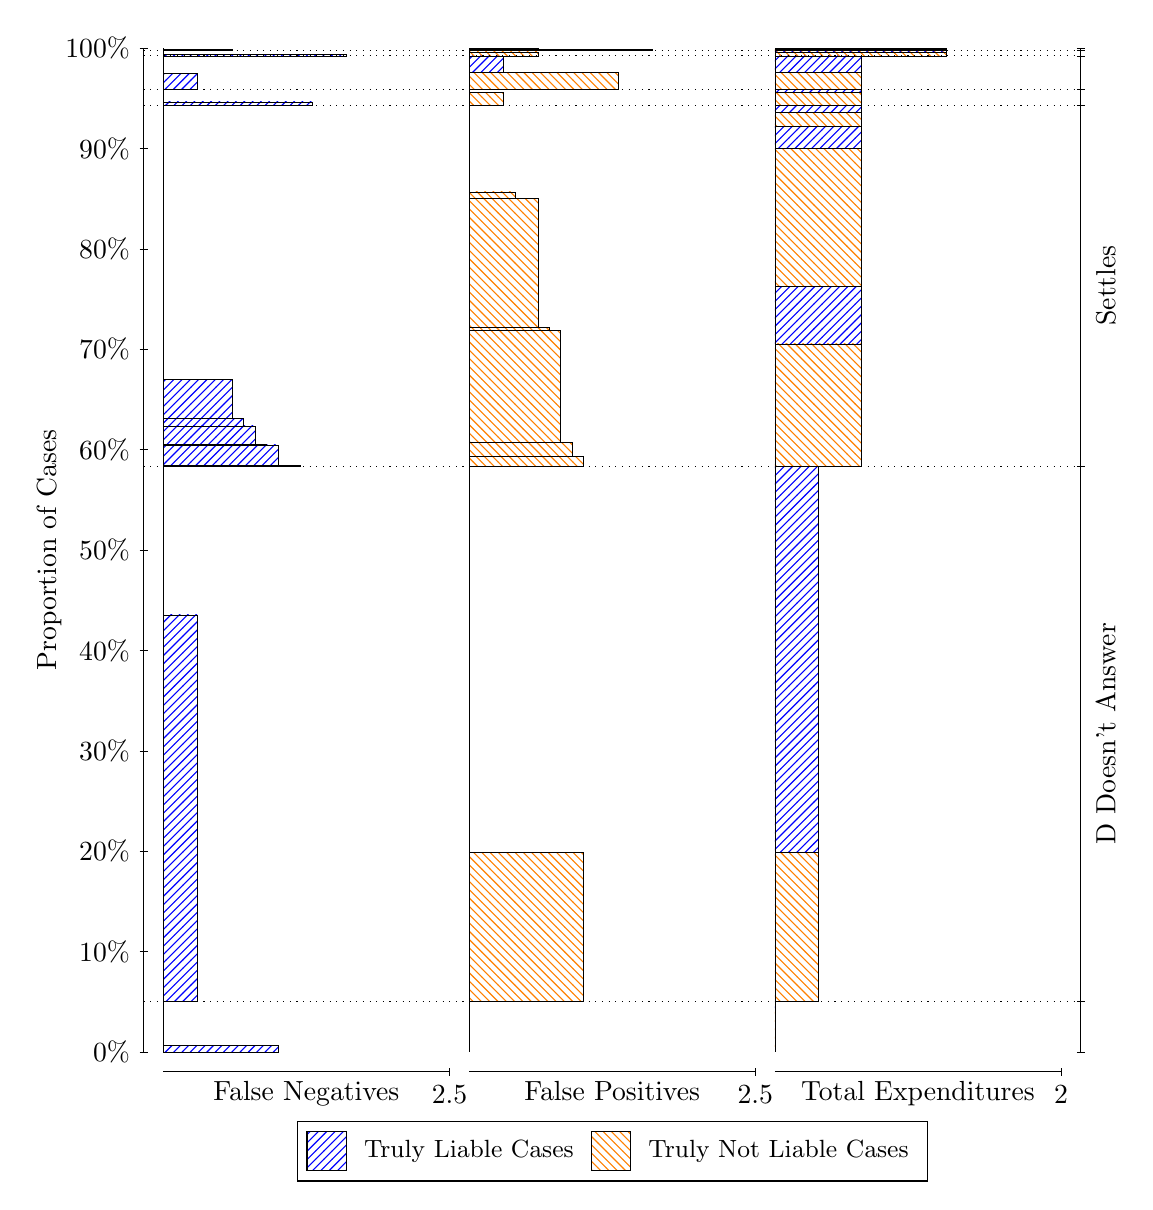
\begin{tikzpicture}
\draw[black, very thin] (1.5,1.75) -- (1.5,14.5);
\node[rotate=90, text=black, anchor=center] at (0.3, 8.125) {Proportion of Cases};
\draw[black, very thin] (1.45,1.75) -- (1.55,1.75);
\node[text=black, anchor=east] at (1.45, 1.75) {0\%};
\draw[black, very thin] (1.45,3.025) -- (1.55,3.025);
\node[text=black, anchor=east] at (1.45, 3.025) {10\%};
\draw[black, very thin] (1.45,4.3) -- (1.55,4.3);
\node[text=black, anchor=east] at (1.45, 4.3) {20\%};
\draw[black, very thin] (1.45,5.575) -- (1.55,5.575);
\node[text=black, anchor=east] at (1.45, 5.575) {30\%};
\draw[black, very thin] (1.45,6.85) -- (1.55,6.85);
\node[text=black, anchor=east] at (1.45, 6.85) {40\%};
\draw[black, very thin] (1.45,8.125) -- (1.55,8.125);
\node[text=black, anchor=east] at (1.45, 8.125) {50\%};
\draw[black, very thin] (1.45,9.4) -- (1.55,9.4);
\node[text=black, anchor=east] at (1.45, 9.4) {60\%};
\draw[black, very thin] (1.45,10.675) -- (1.55,10.675);
\node[text=black, anchor=east] at (1.45, 10.675) {70\%};
\draw[black, very thin] (1.45,11.95) -- (1.55,11.95);
\node[text=black, anchor=east] at (1.45, 11.95) {80\%};
\draw[black, very thin] (1.45,13.225) -- (1.55,13.225);
\node[text=black, anchor=east] at (1.45, 13.225) {90\%};
\draw[black, very thin] (1.45,14.5) -- (1.55,14.5);
\node[text=black, anchor=east] at (1.45, 14.5) {100\%};

\draw[black, very thin] (13.4,1.75) -- (13.4,14.5);
\draw[black, very thin] (13.35,1.75) -- (13.45,1.75);
\node[anchor=west] at (13.35, 1.75) {};
\draw[black, very thin] (13.35,2.392) -- (13.45,2.392);
\node[anchor=west] at (13.35, 2.392) {};
\draw[black, very thin] (13.35,9.1909) -- (13.45,9.1909);
\node[anchor=west] at (13.35, 9.1909) {};
\draw[black, very thin] (13.35,13.775) -- (13.45,13.775);
\node[anchor=west] at (13.35, 13.775) {};
\draw[black, very thin] (13.35,13.975) -- (13.45,13.975);
\node[anchor=west] at (13.35, 13.975) {};
\draw[black, very thin] (13.35,14.4) -- (13.45,14.4);
\node[anchor=west] at (13.35, 14.4) {};
\draw[black, very thin] (13.35,14.467) -- (13.45,14.467);
\node[anchor=west] at (13.35, 14.467) {};
\draw[black, very thin] (13.35,14.5) -- (13.45,14.5);
\node[anchor=west] at (13.35, 14.5) {};

\draw[black, very thin, pattern color=blue, pattern=north east lines] (1.75,1.75) rectangle (3.2033,1.8354);
\draw[black, very thin, pattern color=orange, pattern=north west lines] (1.75,1.8354) rectangle (1.75,2.392);
\draw[black, very thin, pattern color=blue, pattern=north east lines] (1.75,2.392) rectangle (2.186,7.3008);
\draw[black, very thin, pattern color=orange, pattern=north west lines] (1.75,7.3008) rectangle (1.75,9.1909);
\draw[black, very thin, pattern color=blue, pattern=north east lines] (1.75,9.1909) rectangle (3.494,9.2041);
\draw[black, very thin, pattern color=blue, pattern=north east lines] (1.75,9.2041) rectangle (3.2033,9.4596);
\draw[black, very thin, pattern color=blue, pattern=north east lines] (1.75,9.4596) rectangle (3.058,9.4685);
\draw[black, very thin, pattern color=blue, pattern=north east lines] (1.75,9.4685) rectangle (2.9127,9.7008);
\draw[black, very thin, pattern color=blue, pattern=north east lines] (1.75,9.7008) rectangle (2.7673,9.7949);
\draw[black, very thin, pattern color=blue, pattern=north east lines] (1.75,9.7949) rectangle (2.622,10.292);
\draw[black, very thin, pattern color=orange, pattern=north west lines] (1.75,10.292) rectangle (1.75,13.775);
\draw[black, very thin, pattern color=blue, pattern=north east lines] (1.75,13.775) rectangle (3.6393,13.816);
\draw[black, very thin, pattern color=orange, pattern=north west lines] (1.75,13.816) rectangle (1.75,13.975);
\draw[black, very thin, pattern color=blue, pattern=north east lines] (1.75,13.975) rectangle (2.186,14.181);
\draw[black, very thin, pattern color=orange, pattern=north west lines] (1.75,14.181) rectangle (1.75,14.4);
\draw[black, very thin, pattern color=blue, pattern=north east lines] (1.75,14.4) rectangle (4.0753,14.415);
\draw[black, very thin, pattern color=orange, pattern=north west lines] (1.75,14.415) rectangle (1.75,14.467);
\draw[black, very thin, pattern color=blue, pattern=north east lines] (1.75,14.467) rectangle (2.622,14.485);
\draw[black, very thin, pattern color=orange, pattern=north west lines] (1.75,14.485) rectangle (1.75,14.5);
\draw[black, very thin, pattern color=orange, pattern=north west lines] (5.6333,1.75) rectangle (5.6333,2.3065);
\draw[black, very thin, pattern color=blue, pattern=north east lines] (5.6333,2.3065) rectangle (5.6333,2.392);
\draw[black, very thin, pattern color=orange, pattern=north west lines] (5.6333,2.392) rectangle (7.0867,4.2821);
\draw[black, very thin, pattern color=blue, pattern=north east lines] (5.6333,4.2821) rectangle (5.6333,9.1909);
\draw[black, very thin, pattern color=orange, pattern=north west lines] (5.6333,9.1909) rectangle (7.0867,9.3125);
\draw[black, very thin, pattern color=orange, pattern=north west lines] (5.6333,9.3125) rectangle (6.9413,9.4869);
\draw[black, very thin, pattern color=orange, pattern=north west lines] (5.6333,9.4869) rectangle (6.796,10.919);
\draw[black, very thin, pattern color=orange, pattern=north west lines] (5.6333,10.919) rectangle (6.6507,10.951);
\draw[black, very thin, pattern color=orange, pattern=north west lines] (5.6333,10.951) rectangle (6.5053,12.592);
\draw[black, very thin, pattern color=orange, pattern=north west lines] (5.6333,12.592) rectangle (6.2147,12.674);
\draw[black, very thin, pattern color=blue, pattern=north east lines] (5.6333,12.674) rectangle (5.6333,13.775);
\draw[black, very thin, pattern color=orange, pattern=north west lines] (5.6333,13.775) rectangle (6.0693,13.935);
\draw[black, very thin, pattern color=blue, pattern=north east lines] (5.6333,13.935) rectangle (5.6333,13.975);
\draw[black, very thin, pattern color=orange, pattern=north west lines] (5.6333,13.975) rectangle (7.5227,14.194);
\draw[black, very thin, pattern color=blue, pattern=north east lines] (5.6333,14.194) rectangle (6.0693,14.4);
\draw[black, very thin, pattern color=orange, pattern=north west lines] (5.6333,14.4) rectangle (6.5053,14.452);
\draw[black, very thin, pattern color=blue, pattern=north east lines] (5.6333,14.452) rectangle (5.6333,14.467);
\draw[black, very thin, pattern color=orange, pattern=north west lines] (5.6333,14.467) rectangle (7.9587,14.483);
\draw[black, very thin, pattern color=blue, pattern=north east lines] (5.6333,14.483) rectangle (6.5053,14.5);
\draw[black, very thin, pattern color=orange, pattern=north west lines] (9.5167,1.75) rectangle (9.5167,2.3065);
\draw[black, very thin, pattern color=blue, pattern=north east lines] (9.5167,2.3065) rectangle (9.5167,2.392);
\draw[black, very thin, pattern color=orange, pattern=north west lines] (9.5167,2.392) rectangle (10.062,4.2821);
\draw[black, very thin, pattern color=blue, pattern=north east lines] (9.5167,4.2821) rectangle (10.062,9.1909);
\draw[black, very thin, pattern color=orange, pattern=north west lines] (9.5167,9.1909) rectangle (10.607,10.744);
\draw[black, very thin, pattern color=blue, pattern=north east lines] (9.5167,10.744) rectangle (10.607,11.474);
\draw[black, very thin, pattern color=orange, pattern=north west lines] (9.5167,11.474) rectangle (10.607,13.229);
\draw[black, very thin, pattern color=blue, pattern=north east lines] (9.5167,13.229) rectangle (10.607,13.507);
\draw[black, very thin, pattern color=orange, pattern=north west lines] (9.5167,13.507) rectangle (10.607,13.681);
\draw[black, very thin, pattern color=blue, pattern=north east lines] (9.5167,13.681) rectangle (10.607,13.775);
\draw[black, very thin, pattern color=orange, pattern=north west lines] (9.5167,13.775) rectangle (10.607,13.935);
\draw[black, very thin, pattern color=blue, pattern=north east lines] (9.5167,13.935) rectangle (10.607,13.975);
\draw[black, very thin, pattern color=orange, pattern=north west lines] (9.5167,13.975) rectangle (10.607,14.194);
\draw[black, very thin, pattern color=blue, pattern=north east lines] (9.5167,14.194) rectangle (10.607,14.4);
\draw[black, very thin, pattern color=orange, pattern=north west lines] (9.5167,14.4) rectangle (11.697,14.452);
\draw[black, very thin, pattern color=blue, pattern=north east lines] (9.5167,14.452) rectangle (11.697,14.467);
\draw[black, very thin, pattern color=orange, pattern=north west lines] (9.5167,14.467) rectangle (11.697,14.483);
\draw[black, very thin, pattern color=blue, pattern=north east lines] (9.5167,14.483) rectangle (11.697,14.5);
\draw[black, dotted] (1.5,2.392) -- (13.4,2.392);
\draw[black, dotted] (1.5,9.1909) -- (13.4,9.1909);
\draw[black, dotted] (1.5,13.775) -- (13.4,13.775);
\draw[black, dotted] (1.5,13.975) -- (13.4,13.975);
\draw[black, dotted] (1.5,14.4) -- (13.4,14.4);
\draw[black, dotted] (1.5,14.467) -- (13.4,14.467);
\draw[black, very thin] (1.75,1.5) -- (5.3833,1.5);
\node[text=black, anchor=north] at (3.5667, 1.5) {False Negatives};
\draw[black, very thin] (5.3833,1.45) -- (5.3833,1.55);
\node[text=black, anchor=north] at (5.3833, 1.45) {2.5};

\draw[black, very thin] (5.6333,1.5) -- (9.2667,1.5);
\node[text=black, anchor=north] at (7.45, 1.5) {False Positives};
\draw[black, very thin] (9.2667,1.45) -- (9.2667,1.55);
\node[text=black, anchor=north] at (9.2667, 1.45) {2.5};

\draw[black, very thin] (9.5167,1.5) -- (13.15,1.5);
\node[text=black, anchor=north] at (11.333, 1.5) {Total Expenditures};
\draw[black, very thin] (13.15,1.45) -- (13.15,1.55);
\node[text=black, anchor=north] at (13.15, 1.45) {2};


\node[text=black, centered, rotate=90] at (13.72, 5.7914) {D Doesn't Answer};
\node[text=black, centered, rotate=90] at (13.72, 11.483) {Settles};





\draw (7.449999999999999,1.5) node[draw=none] (baseCoordinate) {};
\begin{scope}[align=center]
        \matrix[scale=0.5, draw=black, below=0.5cm of baseCoordinate, nodes={draw}, column sep=0.1cm]{
            \node[rectangle, draw, minimum width=0.5cm, minimum height=0.5cm, pattern color=blue, pattern=north east lines] {}; &
            \node[draw=none, font=\small, text=black] (B) {Truly Liable Cases}; &
            \node[rectangle, draw, minimum width=0.5cm, minimum height=0.5cm, pattern color=orange, pattern=north west lines] {}; &
            \node[draw=none, font=\small, text=black] (B) {Truly Not Liable Cases}; \\
            };
\end{scope}

\end{tikzpicture}
\end{document}